\documentclass[12pt]{article}
\usepackage[left=2cm, right=2cm, top=2cm]{geometry}
\usepackage[utf8]{inputenc} 
\usepackage{mdframed} %For framing the title
\usepackage{graphicx} % to include images
\usepackage{amsmath} % For math mode
\usepackage{mathtools} %for bmatrix*
\usepackage{caption} % For captions
\usepackage{subcaption} % To use caption while using mini page
\usepackage{amssymb} % To use math symbols
\usepackage{multirow} %To combine multiple rows in a table
\usepackage[table]{xcolor} %To color rows / columns in table
\usepackage{titling} %To vertically center the title page
\usepackage{hyperref} %for URL
\usepackage{float} %For [H] in includegraphics
\usepackage[section]{placeins} %PRevents floats before a section
\usepackage{textcomp} %For degree symbol
\usepackage[none]{hyphenat} %To prevent hyphens
\usepackage{array} %for tables
\usepackage{tabu} %tabu tables
\usepackage{caption} % To caption the table



%----------------------------MATLAB TEMPLATE -------------------------------------
\usepackage{listings}
\usepackage{color} %red, green, blue, yellow, cyan, magenta, black, white
\definecolor{mygreen}{RGB}{28,172,0} % color values Red, Green, Blue
\definecolor{mylilas}{RGB}{170,55,241}
%-----------------------------------------------------------------------------------------

\title{ECE 8540 \\ Analysis of Tracking Systems \\ \quad \\
	Assignment 7 \\ Particle Filter}
\author{Vivek Koodli Udupa \\ C12768888}
\date{November 29, 2018 }

%%To make the title page center vertically centered
%\renewcommand\maketitlehooka{\null\mbox{}\vfill}
%\renewcommand\maketitlehookd{\vfill\null}

\begin{document}
\begin{mdframed}
%Displaying Title
%\begin{titlepage}
\maketitle
%\pagenumbering{gobble}% Remove page numbers (and reset to 1)
%\end{titlepage}
\end{mdframed}
\pagenumbering{arabic}% Arabic page numbers (and reset to 1)


%Begin of Report
\section{Introduction}
This report considers the problem of modeling a system described by Hidden Markov Model(HMM). A Markov model is a stochastic model used to model randomly changing systems. A Markov process is a random process where the future state is independent of the past states given the present state. A Hidden Markov Model is a statistical Markov model in which the system being modeled is assumed to be a Markov process with unobserved (i.e. hidden) states. The aim is to discover the hidden state
sequence that most likely describes a given observation sequence. \\

One solution to this problem is to use the Viterbi algorithm, which finds the single best state sequence for an observation sequence. For example, in speech-to-text (speech recognition), the acoustic signal is treated as the observed sequence of events, and a string of text is considered to be the \lq\lq{hidden cause}\rq\rq{} of the acoustic signal. The Viterbi algorithm finds the most likely string of text given the acoustic signal.  \\

The problem considered for this report is a simple HMM which comprises of two states, H(High GC content) and L(Low GC content). State H characterizes coding DNA while state L characterizes non-coding DNA. The model is used to predict the region of coding DNA from two given sequences \lq{GGCACTGAA}\rq{} and \lq{TCAGCGGCT}\rq{}.

\section{Methods}
This section describes the implementation of the Viterbi algorithm to find the hidden state probabilities for the given problem.

\subsection{Description of the HMM}
The HMM in consideration is shown in Figure \ref{fig:HMM}. The model consists of two states, labeled H and L in the example, which can be given numerical values of 0 and 1. The prior probabilities are {0.5, 0.5}. The state transition
probabilities are {0.5, 0.5} for state 0 and {0.4, 0.6} for state 1. Each state observes a discrete value that takes on one of four values {A, C, G, T } that can be given numerical values {0, 1, 2, 3}. The emission probabilities of these values are {0.2, 0.3, 0.3, 0.2} for state 0 and {0.3, 0.2, 0.2, 0.3} for state 1.
 
 \begin{figure}[H]
	\centering
	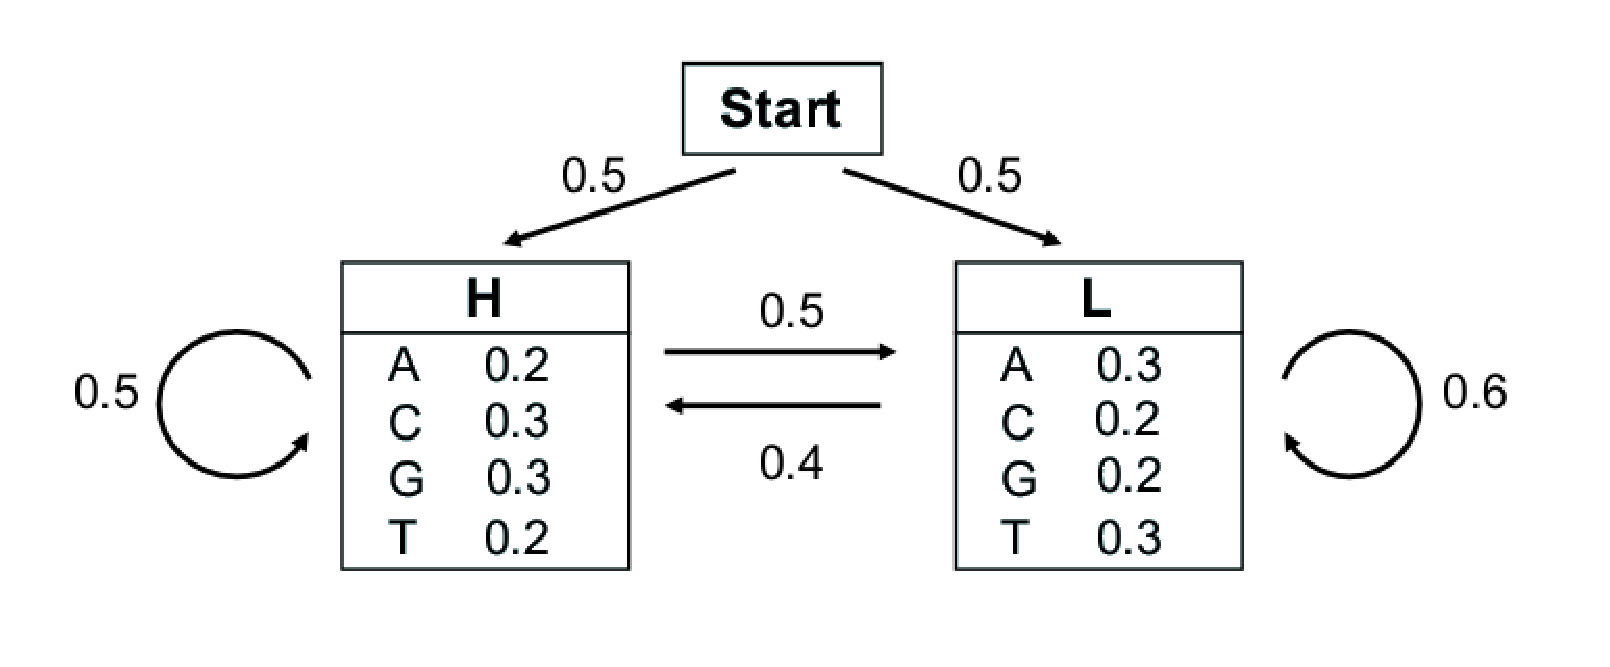
\includegraphics[scale=0.4]{HMM.eps}
	\caption{The Hidden Markov Model with H and L States}
	\label{fig:HMM}
\end{figure}

The Viterbi calculations are done using sums of $log_2$ probabilities.

\subsection{Implementation of Viterbi algorithm}
There are several paths that lead to the desired sequence of states, but not all of them have the same probabilities. The Viterbi algorithm is a dynamical programming algorithm that computes the most probable path. \\

Consider a HMM with k states. The probability of the most probable path ending in state $l$ with observation $i$ is: 
\begin{equation}
	p_l(i,x) = e_l(i) \cdot \displaystyle\max_k(p_k(j,x-1) \cdot p_{kl})
\end{equation}
where $e_l(i)$ is the  probability to observe element i in state l. $p_k(j,x-1)$ is the probability of the most probable path ending at position x-1 in state k with element j. $p_{kl}$ is probability of the transition from state l to state k. \\

For the given sequence \lq\lq{GGCACTGAA}\rq\rq{}, the probability of the most probable path ending in state \lq{H}\rq{} with observation \lq{A}\rq{} at the fourth position (given C at third position) is calculated as:

\begin{equation}
	p_H(A,4) = e_H(A) \cdot max(p_L(C,3) \cdot p_{LH}, p_H(C,3) \cdot p_{HH} )
\end{equation} \\

Similarly the most probably path can be computed recursively from the first to the last element in the given sequence. 

\subsection{Backtracking}
Once the probabilities for all possible states are calculated, the path to the maximum probability is backtracked to find the best path. The state with the highest probability is chosen. In cases where both the states have the same probability value, same path as the previous state is maintained. 

\section{Results}
This sections consists of the results i.e. the table of max probabilities obtained from the Viterbi algorithm for the two given sequences. The calculation was done using $log_2$ of probabilities. \\

\subsection{Input Sequence 1} 
\begin{center}
\begin{tabular}{ | m{5em} | m{3em} | m{3em} | m{3em} | m{3em} | m{3em} | m{3em} | m{3em} | m{3em} | m{3em} | }
 \hline
 Input Sequence & G & G & C & A & C & T & G & A & A \\
 \hline
 State H & \textbf{-2.73} & \textbf{-5.47} & \textbf{-8.21} & -11.53 & -14.00 & -17.32 & -19.53 & -22.86 & -25.65  \\
 \hline
 State L & -3.32 & -6.05 & -8.79 & \textbf{-10.94} & \textbf{-14.00} & \textbf{-16.48} & \textbf{-19.53} & \textbf{-22.01} & \textbf{-24.48} \\
 \hline
 Best Path & H & H & H & L & L & L & L & L & L \\
 \hline
\end{tabular}
\captionof{table}{Table of maximum probabilities for sequence \lq\lq{GGCACTGAA}\rq\rq{} }
\label{Table:1}
\end{center}

Table \ref{Table:1} shows the best probable path for the given sequence \lq\lq{GGCACTGAA}\rq\rq{} is HHHLLLLLL and the maximum probability is $2^{-24.48}$ = $4.2517\times10^{-08}$. The boldfaced numbers represent the highest probability for that particular event.

\subsection{Input Sequence 2} 

\begin{center}
\begin{tabular}{ | m{5em} | m{3em} | m{3em} | m{3em} | m{3em} | m{3em} | m{3em} | m{3em} | m{3em} | m{3em} | }
 \hline
 Input Sequence & T & C & A & G & C & G & G & C & T \\
 \hline
 State H & -3.32 & -5.79 & -9.11 & \textbf{-11.32} & \textbf{-14.06} & \textbf{-16.80} & \textbf{-19.53} & \textbf{-22.27} & -25.59  \\
 \hline
 State L & \textbf{-2.73} & \textbf{-5.79} & \textbf{-8.26} & -11.32 & -14.38 & -17.38 & -20.12 & -22.86 & \textbf{-25.01} \\
 \hline
 Best Path & L & L & L & H & H & H & H & H & L \\
 \hline
\end{tabular}
\captionof{table}{Table of maximum probabilities for sequence \lq\lq{TCAGCGGCT}\rq\rq{} }
\label{Table:2}
\end{center}

Table \ref{Table:2} shows the best probable path for the given sequence \lq\lq{TCAGCGGCT}\rq\rq{} is LLLHHHHHL and the maximum probability is $2^{-25.01}$ = $2.9525\times10^{-08}$. The boldfaced numbers represent the highest probability for that particular event. 

\section{Conclusion}
The Viterbi algorithm is used to compute the most probable path (as well as its probability). It requires knowledge of the parameters of the HMM model and a particular output sequence and it finds the state sequence that is most likely to have generated that output sequence. It works by finding a maximum over all possible state sequences. \\

There are often many state sequences that can produce the same particular output sequence, but with different probabilities. It is possible to calculate the probability for the HMM model to generate that output sequence by doing the summation over all possible state sequences. 

\section*{References}
[1] \url {https://en.wikipedia.org/wiki/Viterbi_algorithm} \\
\\ \noindent
[2] \url {https://en.wikipedia.org/wiki/Hidden_Markov_model} \\
\\ \noindent
[3] \url {http://cecas.clemson.edu/~ahoover/ece854/} \\
\section*{Appendix}

\subsection*{Main}
\lstinputlisting{../Code/run.m}
\subsection*{Viterbi algorithm implementation}
\lstinputlisting{../Code/Viterbi.m}
\subsection*{Backtracking}
\lstinputlisting{../Code/Backtracking.m}
\subsection*{Conversion}
\lstinputlisting{../Code/Convert.m}

%--------------------------------------------------------------------------------------------------------

\end{document}